\documentclass{article}
\usepackage[utf8]{inputenc}
\usepackage{graphicx}
\setlength{\parindent}{0pt}
\setlength{\parskip}{1em}

\title{FOAR705 - Learning Journal - Elaboration}
\author{Jan Jugueta - 44828020}
\date{August \& September 2019}

\begin{document}

\maketitle

\section*{26/8/19 - 10:21am}

One of the pains I regularly experience when doing academic work is that I am very poor at time management. I spend alot of time trying to remember where I found a particular quote, or which source I got an idea from. It doesn't help that I am not sure exactly what I'll be doing for my MRes project. I have some ideas, but I don't have \textit{the} idea.

\section*{26/8/19 - 3:15pm}

I just finished meeting Dr. Norbert Ebert. He was my lecturer for the Social Theory class I did in semester one. My supervisor is currently away in Germany on study leave so I thought it would be a good idea to meet with him and get some advice regarding my MRes project. I explained to him that I was torn between different ideas, some ideas I was more passionate about, whilst others were more practical. The advice he gave was that I should choose the more practical topic. The rationale behind it was that an MRes thesis is very short. I had  ambitious ideas regarding what I want to do and I conceded the fact that it be better suited to a PhD project. He also said that the research that I carry out can and should be used as a springboard onto a PhD.

So now I have resolved myself to a definitive topic. It will involve analysing the way that the East German state were portraying the first (and only) football match between East and West Germany. Of particular significance was the fact that this football match would take place in West Germany, during the World Cup Finals. Newspaper articles from \textit{Neues Deutschland} would be my primary source for the research.

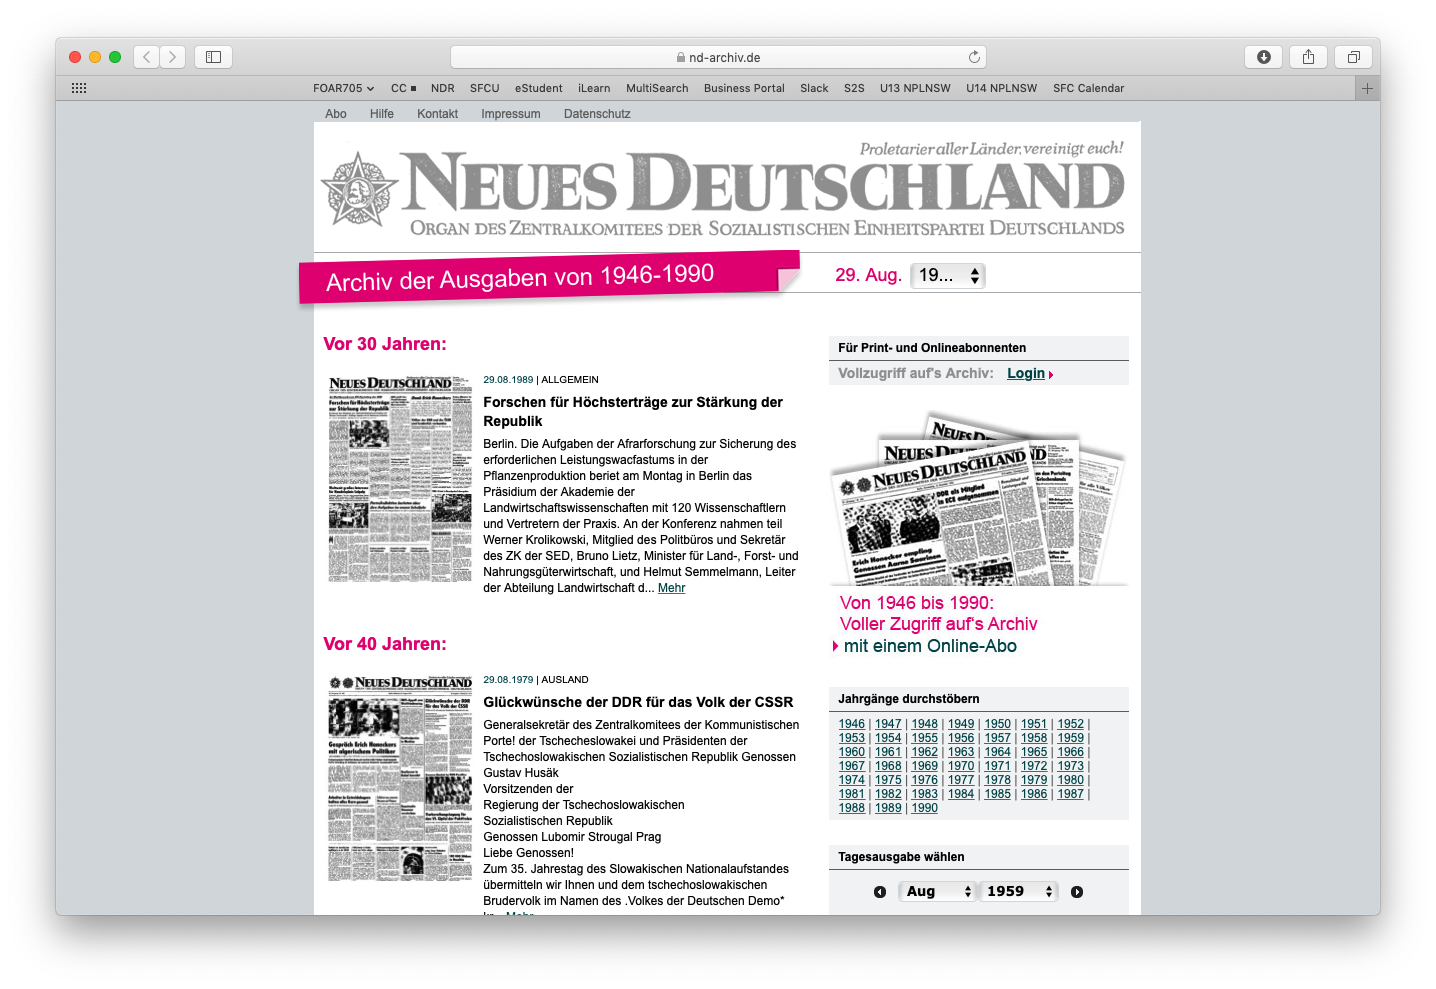
\includegraphics[width=\textwidth]{nd.png}

\section*{26/8/19 - 5:29pm}

With a clearer idea of what I want to do in my MRes project, I would probably need to redefine some things I had outlined in my Scoping exercise.

\subsection*{Decomposition}

\begin{itemize}
    \item Collect newspaper articles from \textit{Neues Deutschland}
    \item Store them on my computer
    \item Find a way to analyse the text
    \item Write notes on my findings
\end{itemize}

Although the above is very rudimentary, it is a rough outline of the stages I will need to go through when doing my research.

\section*{28/8/19 - 8:53pm}

I had emailed my supervisor Dr. Ulrike Garde about the status of my MRes project. She was happy that I had finally gained some clarity around what my project would be. It was always going to be about football and Germany. It was just a question of how these two concepts could fit together.

\section*{29/8/19 - 1:21pm}

I will now see if \textit{Neues Deutschland} has any articles about the 1974 World Cup in West Germany.

\textbf{Objective:} Find out if \textit{Neues Deutschland} has articles about the 1974 FIFA World Cup.

\textbf{Action:}
\begin{itemize}
    \item Go to the website www.nd-archiv.de
    \item Go to the bottom right hand corner where it says \textit{Archiv durchsuchen} (lit. Archive search through)
    \item Type in \textit{Weltmeisterschaft} (lit. World Championships)
\end{itemize}

\textbf{Error:} None

\textbf{Result:} There are some articles about the World Cup. However, it is showing articles from before and after the 1974 World Cup.

\section*{29/8/19 - 1:25pm}

After the previous search, a new advanced search appeared at the bottom of the search results. This advanced search gives the user the ability to specify a time range.

\textbf{Objective:} Find out if \textit{Neues Deutschland} has articles about the 1974 FIFA World Cup by restricting the date range to the years of 1973 and 1974.

\textbf{Action:}
\begin{itemize}
    \item Go to the website www.nd-archiv.de
    \item Use the advanced search option 
    \item Type in \textit{Weltmeisterschaft} (lit. World Championships) in the \textit{Suchausdruck} (lit. search expression)
    \item In the \textit{In welchem Zeitraum} restrict the search from 1/1/1973 to 31/12/1974
    \item Leave all other options in their default settings
\end{itemize}

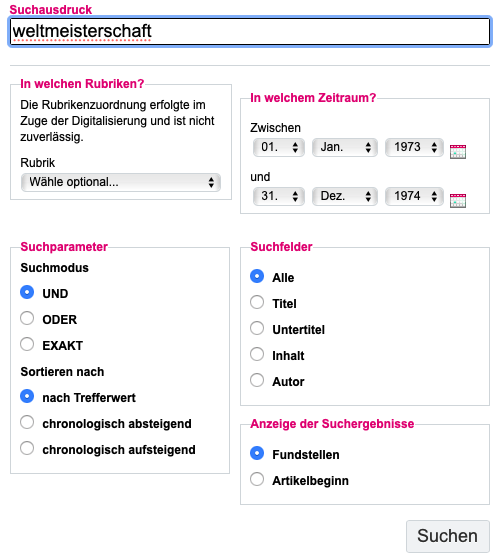
\includegraphics[width=\textwidth]{nd_search.png}

\textbf{Error:} None

\textbf{Result:} The search result returned articles only from 1973 and 1974. However, it does return results from other sports' World Cups. I have considered adding the term \textit{Fußball} in the search query, but I think it may rule out articles that do not specifically mention football in the article, but are still about the FIFA World Cup.

\section*{29/8/19 - 2:05pm}

Now that I know I have sources I can use, the next step is to find out whether Voyant Tools can analyse German text. I remember a discussion in class about Voyant Tools being used as a textual analysis tool. I also remember a former classmate talking about how they used it for their semiotic analysis of text. The web address is www.voyant-tools.org.

\section*{29/8/19 - 2:11pm}

\textbf{Objective:} Find out if Voyant Tools can analyse German text.

\textbf{Action:}

\begin{itemize}
    \item Copied the entirety of Marx's \textit{Manifest der Kommunistischen Partei}
    \item Pasted the text in the Voyant Tools text box
    \item Clicked reveal
\end{itemize}

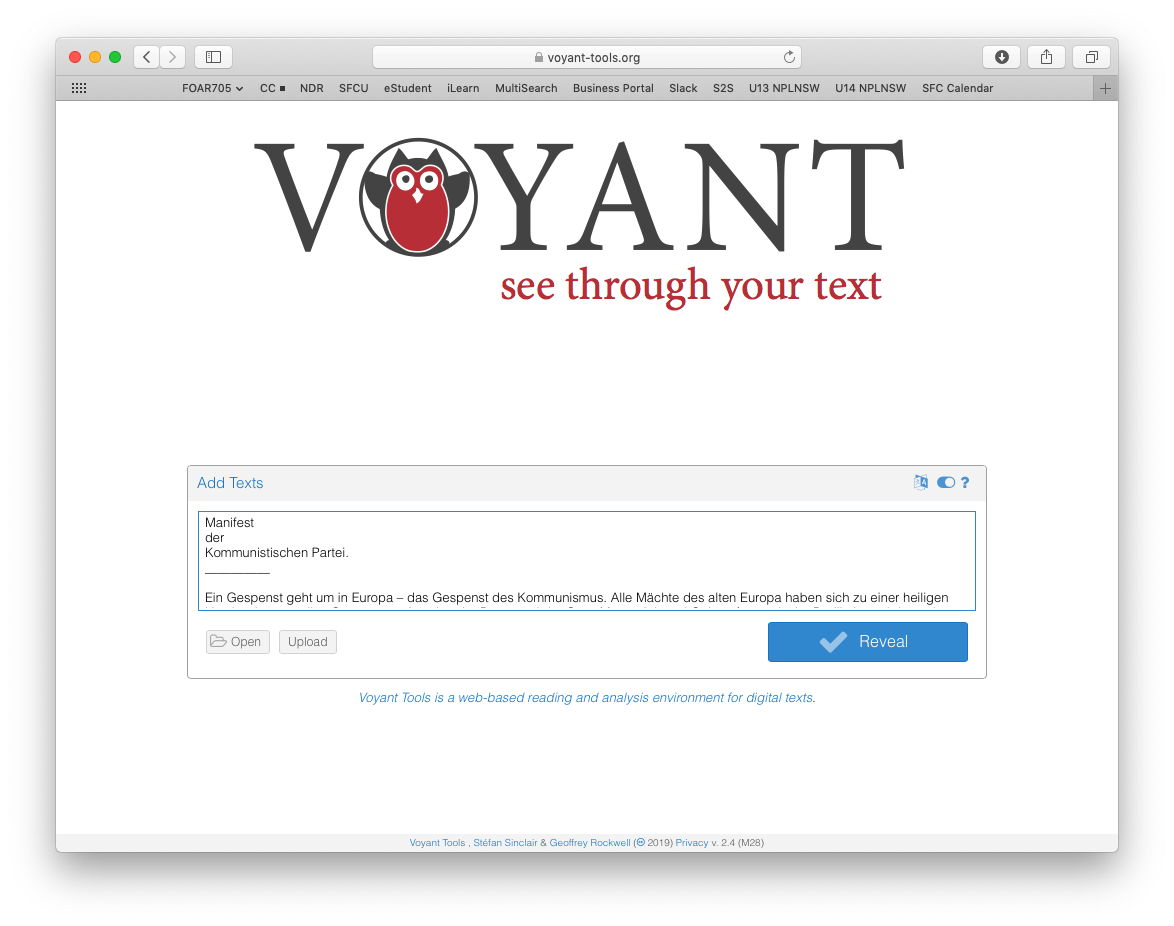
\includegraphics[width=\textwidth]{vtkommunismus.png}

\textbf{Error:} None.

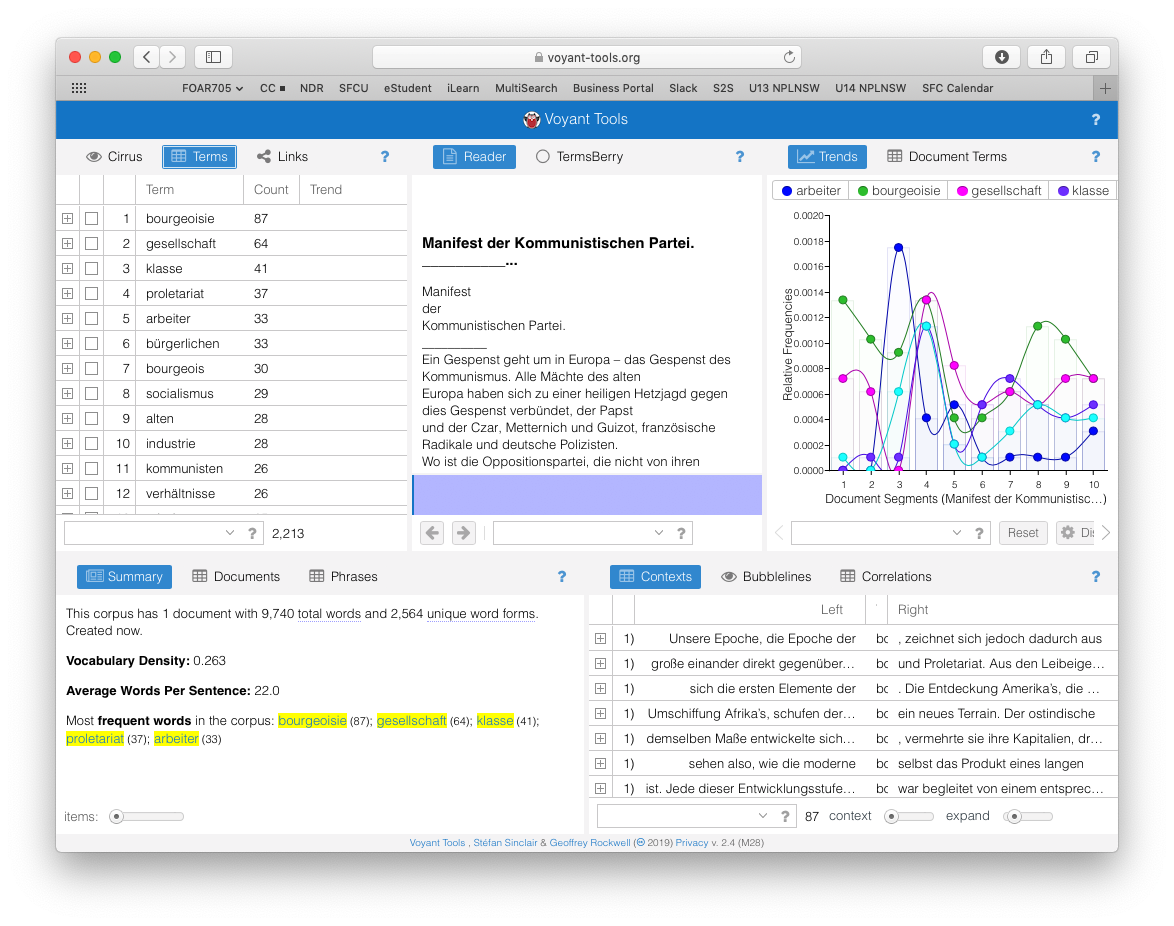
\includegraphics[width=\textwidth]{bourgeoisie.png}

\textbf{Result:} Voyant Tools indeed does work with German. It is also unsurprising that the most common word in the Communist Manifesto is \textit{bourgeoisie}.

\section*{29/8/19 - 2:29pm}

Now that I know Voyant Tools can work with German text, my next question is whether it can work with a corpus of text. This will require saving numerous articles on my machine ready to be analysed.

\textbf{Objective:} Save three articles from \textit{Neues Deutschland}.

\textbf{Action:} 

\begin{itemize}
    \item Performed \textit{Weltmeisterschaft} search within the years of 1973 and 1974
    \item Entered the first article that was returned in the search
    \item Copied the text of the article
    \item Opened Text Edit on my machine
    \item Pasted the article
    \item Saved the article with the naming convention 'nd\_yearmonthday' with the with a letter appendage signifying difference if there were multiple articles published on the same day
    \item Article saved under 'nd\_19740721a.rtf in textfiles folder
    \item Repeated this process of copying, naming and saving the next two articles
\end{itemize}

\textbf{Error:} None.

\textbf{Result:} Three articles successfully saved as .rtf files.

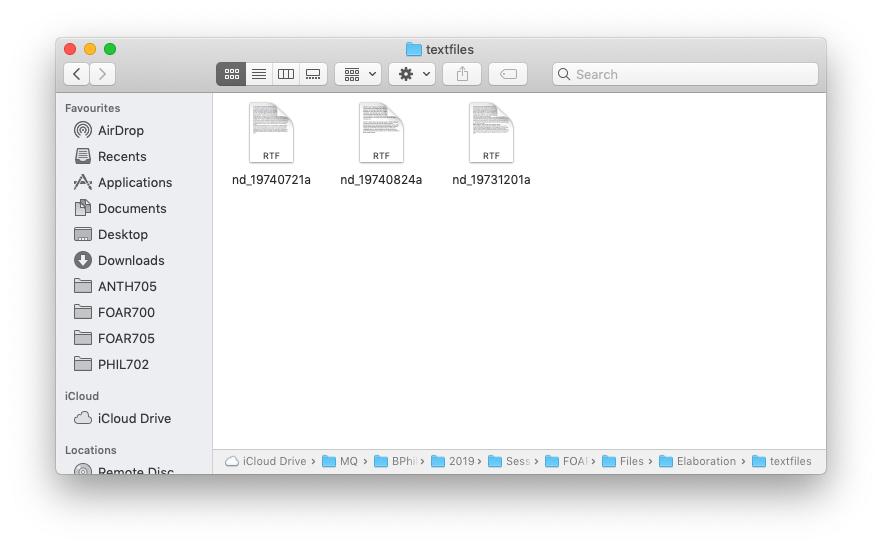
\includegraphics[width=\textwidth]{textfiles.png}

\section*{29/8/19 - 2:46pm}

Now that I have three .rtf files, I want to see if Voyant Tools can accept all three in an upload.

\textbf{Objective:} Upload three .rtf files into Voyant Tools

\textbf{Action:}

\begin{itemize}
    \item Go to www.voyant-tools.org
    \item Select the upload option
    \item Navigate to the textfiles folder
    \item Selected the three .rtf files
    \item Click on choose
\end{itemize}

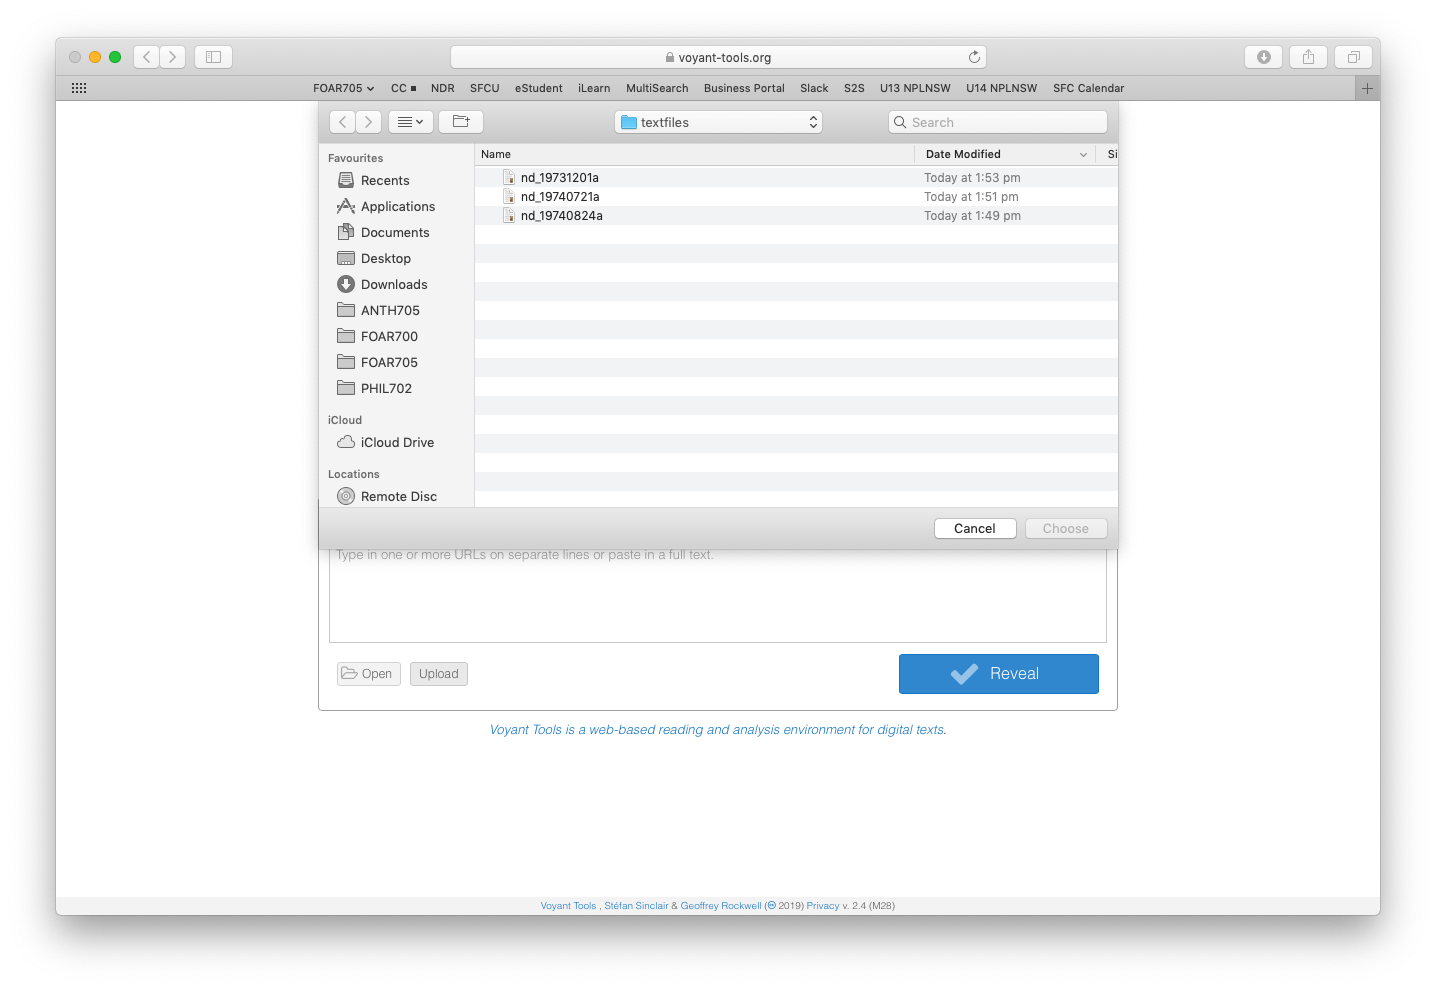
\includegraphics[width=\textwidth]{voyantupload.png}

\textbf{Error:} None.

\textbf{Result:} Voyant Tools can indeed analyse text from a number of .rtf files.

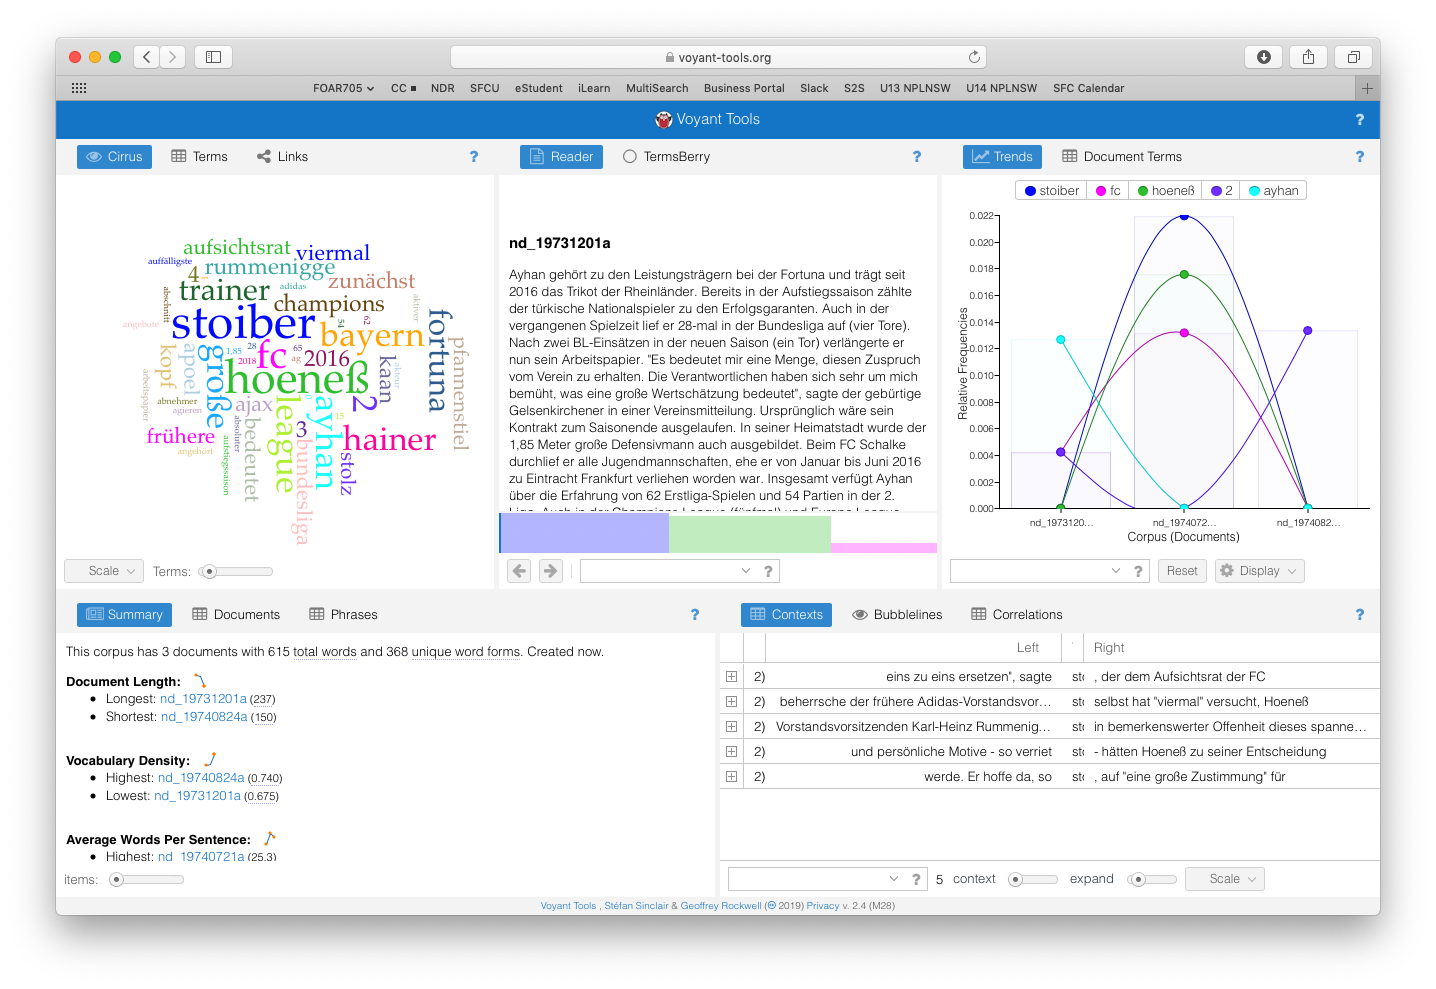
\includegraphics[width=\textwidth]{voyantresult.png}

\section*{31/8/19 - 10:12am}

Reflecting on our last meeting in FOAR705, I recall discussion around APIs and how they can help with collecting data. As my current workflow of copying articles and pasting them in Text Edit requires me to manually do one article at a time, I wondered if there was an API available.

\section*{31/8/19 - 10:32am}

After some searching, there is \textbf{no API available} for the \textit{Neues Deutschland} archive. It seems that I will have to continue copying the articles manually.

\section*{1/9/19 - 11:01am}

Revisiting my Elaboration I document, I realise that I probably need to rewrite some of the work I did for Scoping. This includes what is part of my Decomposition, Pattern Recognition and Algorithm.

\section*{1/9/19 - 1:27pm}

After sitting down for some time with a pen and a pad, I was able to mind map what would be involved in this research process. Listed below are the individual items that comprise my research workflow.

\begin{itemize}
    \item identifying a date search range
    \item identifying key search terms
    \item sorting out irrelevant news articles
    \item downloading the text from the newspaper articles onto my machine
    \item storing the articles in a directory on my machine
    \item labelling and tagging articles for ease of re-use
    \item uploading the articles to a text analysis website
    \item interpreting the textual analysis
    \item identify key themes from the analysis
\end{itemize}

\section*{1/9/19 - 3:45pm}

I have a better understanding of what Pattern Recognition means. I previously thought it meant what type of patterns my software solution could recognise. This was then reflected in my Scoping I exercise. I now conceive of Pattern Recognition as the processes that would often be repeated in my research. Below are the list of patterns that I have recognised.

\begin{itemize}
    \item the repetition of the search process when using a new search term (including the sorting out of irrelevant articles, downloading articles and storing them in a directory)
    \item the repetition of the process to uploading the articles to a world analysis website
    \item the repetition of the process to log and key findings that may emerge from the textual analysis
\end{itemize}

\section*{1/9/19 - 6:19pm}

After spending some time away from my computer, I was able to brainstorm again on the good ol' real life note pad. This gave me the ability to figure out what my algorithm looked like. Below is what I came up with.

\begin{enumerate}
    \item Access web archive of the newspaper
    \item Delimit search time period (i.e. 1/1/1973 - 31/12/1974)
    \item Enter search term in the search window
    \item Sort out relevant and irrelevant newspaper articles
    \item Download (or copy) the text from the newspaper article
    \item Save the text onto a .txt file on my machine
    \item Tag metadata information of the article including publish date, authors name and location
    \item Organise articles by date (or theme, I have not yet decided which is best)
    \item Upload the corpus of text to textual analysis website
    \item Identify themes that emerge from the analysis
    \item Note down findings in research journal.
\end{enumerate}

\section*{4/9/19 - 12:53pm}

Revisiting Elaboration I, I recognised that I had mentioned that I will take notes of what I found in Voyant Tools, but did not actually mention this process. I currently use Microsoft OneNote for my note taking in all my university subjects and have done so since my first year as an undergraduate. OneNote has been an integral part of my workflow in academic work.

\section*{4/9/19 - 1:08pm}

I want to know how OneNote can help me organise my notes for my MRes project. This use of OneNote will be different than my previous uses because I only had one workbook, with one section for each of the units I studied.

OneNote gives the user the ability to have multiple sections in a workbook, which then contain multiple pages. To conceive of a way to organise my notes, I thought of note categories I could use.

\begin{itemize}
    \item Key Concepts
    \item Notes from Literature
    \item Notes from primary sources
    \item Misc ideas
\end{itemize}

\section*{5/9/19 - 12:43pm}

\textbf{Objective:} Create sections for the different note categories in OneNote

\textbf{Action:}

\begin{itemize}
    \item Added section
    \item Named new section Key Concepts
    \item Added section
    \item Named new section Notes from Literature
    \item Added section
    \item Named new section Notes from primary sources
    \item Added section
    \item Named new section Misc ideas
\end{itemize}

\textbf{Error:} None.

\textbf{Result:} New sections created in OneNote that correspond to the note categories.

\section*{5/9/19 - 1:31pm}

I just finished a YouTube video about OneNote. One feature that I had not used yet was the Tag feature. I do not yet want to add the Tagging feature as part of this elaboration as I have not yet figure out how I would use it. It is nice to know I have that feature if I want it.

\section*{5/9/19 - 1:39pm}

After watching that video, I also had a lightbulb moment. It regards to back ups. I had learnt that OneNote is based entirely off their cloud, with no offline save option. This could be hazardous if the cloud is somehow corrupted.

\section*{5/9/19 - 1:45pm}

Now worrying about potential data loss, I have been thinking about other note taking solutions. I have consider two others:
\begin{enumerate}
    \item Microsoft Word
    \item Text files
\end{enumerate}

Both would require me writing notes in a new document every single time and saving them to a directory on my machine. This would then require me to manage the file structure of my notes and I would lose the sync workflow that I use so much between my devices.

\section*{5/9/19 - 1:51pm}

I want to explore the possibility of using .txt files as a means of writing my notes. This is inspired by the work we've been doing in Software Carpentry. It also allows for shell use in the future.

\section*{5/9/19 - 2:02pm}

\textbf{Objective:} Copy my notes that I have from different places and store them as .txt files in a directory on my machine.

\textbf{Action:}
\begin{itemize}
    \item Copy notes from Gupta - Nationalism.docx
    \item Open Text Edit
    \item Go to Format menu
    \item Select Make Rich Text
    \item Paste text
    \item Save file as gupta-nationalism.txt in articles directory
    \item Repeat process for other article notes
\end{itemize}

\textbf{Error:} None.

\textbf{Result:} Notes are now in .txt format.

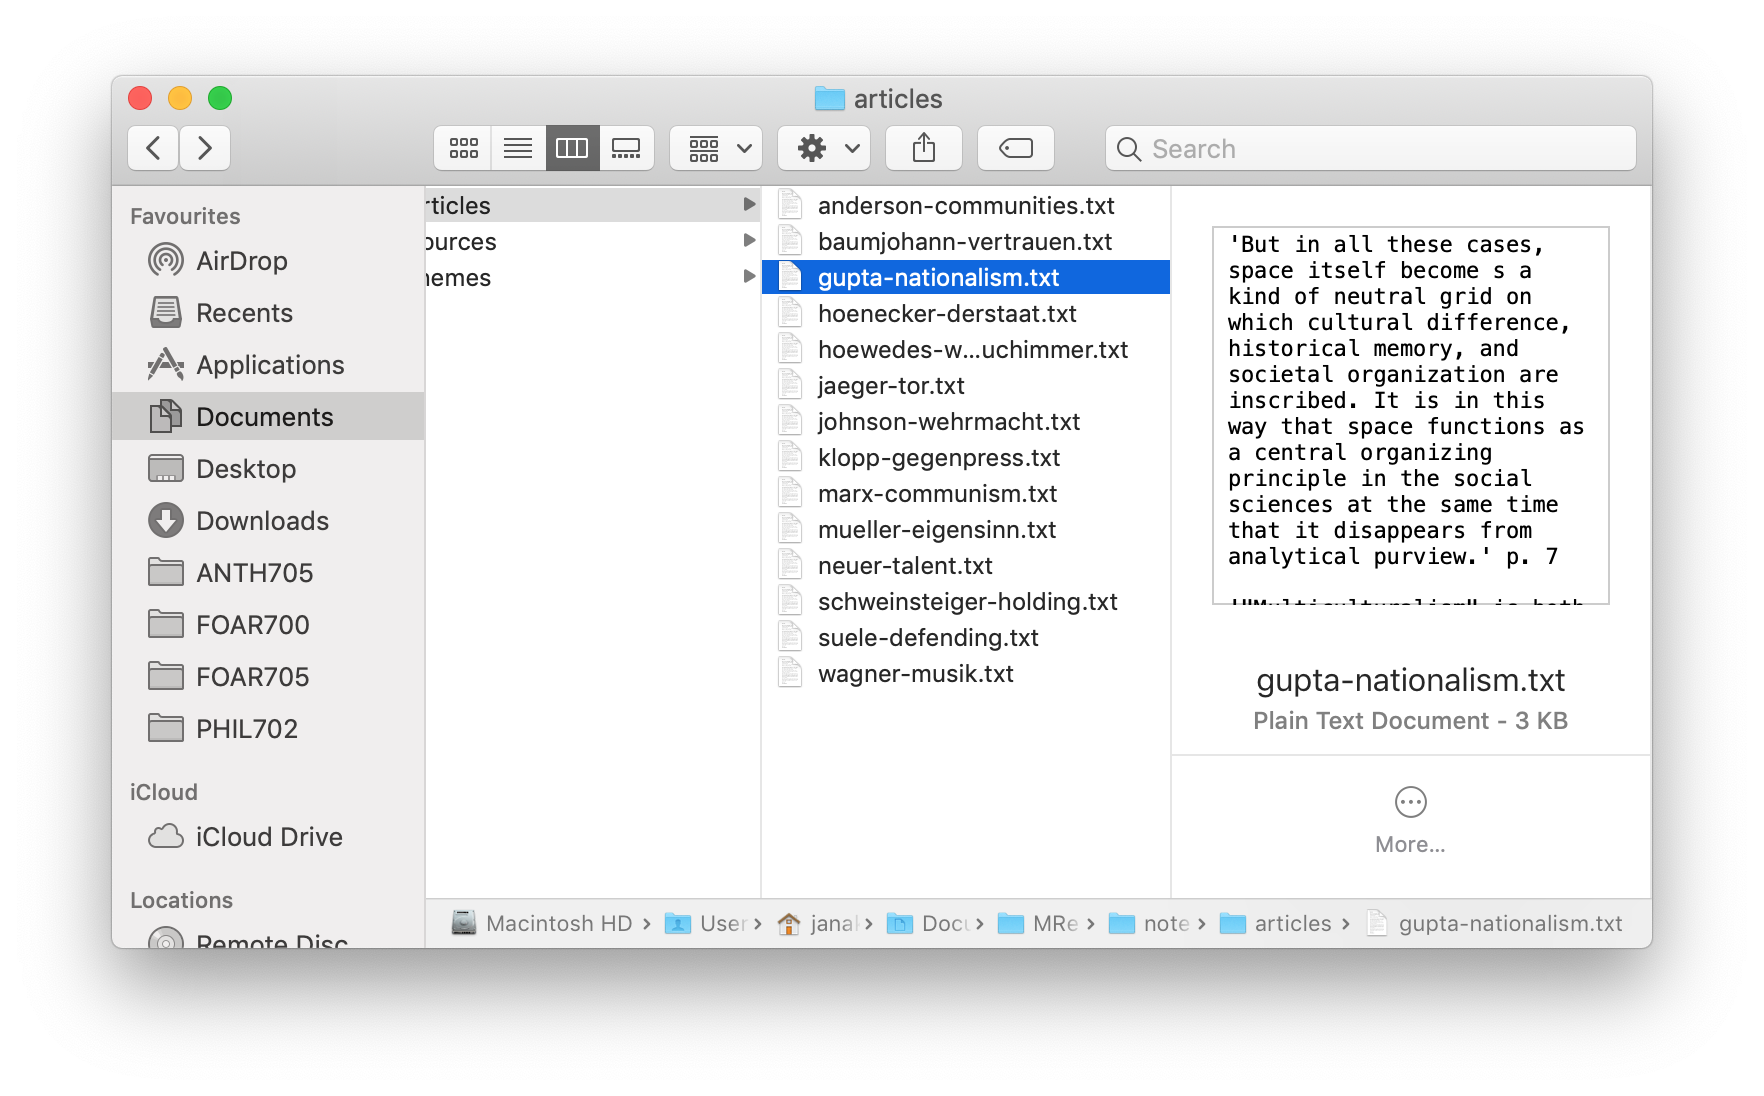
\includegraphics[width=\textwidth]{text.png}

\section*{5/9/19 - 2:25pm}

Having these notes saved as .txt files means I can commit notes to GitHub. Now I need to choose which way I will go.

\section*{5/9/19 - 2:29pm}

I think I will still use OneNote. I'm a creature of habit. However, I will keep on looking for back up options that work with OneNote.

\section*{5/9/19 - 10:30pm}

Some final thoughts about this Elaboration assessment. I am not sure if the Proof of Concepts I have chosen are complex enough. What has guided me through this process have been two main criteria:
\begin{itemize}
    \item Is it achievable in a short time?
    \item Will it help my workflow
\end{itemize}

What I have proposed satisfies both. It also allows me to build on this as a platform. I will continue to look at ways to economize the way I work.

\end{document}
